\documentclass[conference]{IEEEtran}
% \documentclass[conference]{../sty/IEEEtran}

% *** CITATION PACKAGES ***
%
%\usepackage{cite}
% cite.sty was written by Donald Arseneau
% V1.6 and later of IEEEtran pre-defines the format of the cite.sty package
% \cite{} output to follow that of the IEEE. Loading the cite package will
% result in citation numbers being automatically sorted and properly
% "compressed/ranged". e.g., [1], [9], [2], [7], [5], [6] without using
% cite.sty will become [1], [2], [5]--[7], [9] using cite.sty. cite.sty's
% \cite will automatically add leading space, if needed. Use cite.sty's
% noadjust option (cite.sty V3.8 and later) if you want to turn this off
% such as if a citation ever needs to be enclosed in parenthesis.
% cite.sty is already installed on most LaTeX systems. Be sure and use
% version 5.0 (2009-03-20) and later if using hyperref.sty.
% The latest version can be obtained at:
% http://www.ctan.org/pkg/cite
% The documentation is contained in the cite.sty file itself.

% *** GRAPHICS RELATED PACKAGES ***
%
\ifCLASSINFOpdf
   \usepackage[pdftex]{graphicx}
  % declare the path(s) where your graphic files are
  % \graphicspath{{../pdf/}{../jpeg/}}
  % and their extensions so you won't have to specify these with
  % every instance of \includegraphics
  % \DeclareGraphicsExtensions{.pdf,.jpeg,.png}
\else
  % or other class option (dvipsone, dvipdf, if not using dvips). graphicx
  % will default to the driver specified in the system graphics.cfg if no
  % driver is specified.
   \usepackage[dvips]{graphicx}
  % declare the path(s) where your graphic files are
  % \graphicspath{{../eps/}}
  \graphicspath{ {./img/} }
  % and their extensions so you won't have to specify these with
  % every instance of \includegraphics
  % \DeclareGraphicsExtensions{.eps}
\fi
\graphicspath{ {./img/} }
% graphicx was written by David Carlisle and Sebastian Rahtz. It is
% required if you want graphics, photos, etc. graphicx.sty is already
% installed on most LaTeX systems. The latest version and documentation
% can be obtained at: 
% http://www.ctan.org/pkg/graphicx
% Another good source of documentation is "Using Imported Graphics in
% LaTeX2e" by Keith Reckdahl which can be found at:
% http://www.ctan.org/pkg/epslatex
%
% latex, and pdflatex in dvi mode, support graphics in encapsulated
% postscript (.eps) format. pdflatex in pdf mode supports graphics
% in .pdf, .jpeg, .png and .mps (metapost) formats. Users should ensure
% that all non-photo figures use a vector format (.eps, .pdf, .mps) and
% not a bitmapped formats (.jpeg, .png). The IEEE frowns on bitmapped formats
% which can result in "jaggedy"/blurry rendering of lines and letters as
% well as large increases in file sizes.
%
% You can find documentation about the pdfTeX application at:
% http://www.tug.org/applications/pdftex

% *** MATH PACKAGES ***
%
%\usepackage{amsmath}
% A popular package from the American Mathematical Society that provides
% many useful and powerful commands for dealing with mathematics.
%
% Note that the amsmath package sets \interdisplaylinepenalty to 10000
% thus preventing page breaks from occurring within multiline equations. Use:
%\interdisplaylinepenalty=2500
% after loading amsmath to restore such page breaks as IEEEtran.cls normally
% does. amsmath.sty is already installed on most LaTeX systems. The latest
% version and documentation can be obtained at:
% http://www.ctan.org/pkg/amsmath


% *** SPECIALIZED LIST PACKAGES ***
%
\usepackage{algorithmic}
% algorithmic.sty was written by Peter Williams and Rogerio Brito.
% This package provides an algorithmic environment fo describing algorithms.
% You can use the algorithmic environment in-text or within a figure
% environment to provide for a floating algorithm. Do NOT use the algorithm
% floating environment provided by algorithm.sty (by the same authors) or
% algorithm2e.sty (by Christophe Fiorio) as the IEEE does not use dedicated
% algorithm float types and packages that provide these will not provide
% correct IEEE style captions. The latest version and documentation of
% algorithmic.sty can be obtained at:
% http://www.ctan.org/pkg/algorithms
% Also of interest may be the (relatively newer and more customizable)
% algorithmicx.sty package by Szasz Janos:
% http://www.ctan.org/pkg/algorithmicx


% *** ALIGNMENT PACKAGES ***
%
%\usepackage{array}
% Frank Mittelbach's and David Carlisle's array.sty patches and improves
% the standard LaTeX2e array and tabular environments to provide better
% appearance and additional user controls. As the default LaTeX2e table
% generation code is lacking to the point of almost being broken with
% respect to the quality of the end results, all users are strongly
% advised to use an enhanced (at the very least that provided by array.sty)
% set of table tools. array.sty is already installed on most systems. The
% latest version and documentation can be obtained at:
% http://www.ctan.org/pkg/array


% IEEEtran contains the IEEEeqnarray family of commands that can be used to
% generate multiline equations as well as matrices, tables, etc., of high
% quality.




% *** SUBFIGURE PACKAGES ***
%\ifCLASSOPTIONcompsoc
%  \usepackage[caption=false,font=normalsize,labelfont=sf,textfont=sf]{subfig}
%\else
%  \usepackage[caption=false,font=footnotesize]{subfig}
%\fi
% subfig.sty, written by Steven Douglas Cochran, is the modern replacement
% for subfigure.sty, the latter of which is no longer maintained and is
% incompatible with some LaTeX packages including fixltx2e. However,
% subfig.sty requires and automatically loads Axel Sommerfeldt's caption.sty
% which will override IEEEtran.cls' handling of captions and this will result
% in non-IEEE style figure/table captions. To prevent this problem, be sure
% and invoke subfig.sty's "caption=false" package option (available since
% subfig.sty version 1.3, 2005/06/28) as this is will preserve IEEEtran.cls
% handling of captions.
% Note that the Computer Society format requires a larger sans serif font
% than the serif footnote size font used in traditional IEEE formatting
% and thus the need to invoke different subfig.sty package options depending
% on whether compsoc mode has been enabled.
%
% The latest version and documentation of subfig.sty can be obtained at:
% http://www.ctan.org/pkg/subfig



% *** FLOAT PACKAGES ***
%
%\usepackage{fixltx2e}
% fixltx2e, the successor to the earlier fix2col.sty, was written by
% Frank Mittelbach and David Carlisle. This package corrects a few problems
% in the LaTeX2e kernel, the most notable of which is that in current
% LaTeX2e releases, the ordering of single and double column floats is not
% guaranteed to be preserved. Thus, an unpatched LaTeX2e can allow a
% single column figure to be placed prior to an earlier double column
% figure.
% Be aware that LaTeX2e kernels dated 2015 and later have fixltx2e.sty's
% corrections already built into the system in which case a warning will
% be issued if an attempt is made to load fixltx2e.sty as it is no longer
% needed.
% The latest version and documentation can be found at:
% http://www.ctan.org/pkg/fixltx2e


%\usepackage{stfloats}
% stfloats.sty was written by Sigitas Tolusis. This package gives LaTeX2e
% the ability to do double column floats at the bottom of the page as well
% as the top. (e.g., "\begin{figure*}[!b]" is not normally possible in
% LaTeX2e). It also provides a command:
%\fnbelowfloat
% to enable the placement of footnotes below bottom floats (the standard
% LaTeX2e kernel puts them above bottom floats). This is an invasive package
% which rewrites many portions of the LaTeX2e float routines. It may not work
% with other packages that modify the LaTeX2e float routines. The latest
% version and documentation can be obtained at:
% http://www.ctan.org/pkg/stfloats
% Do not use the stfloats baselinefloat ability as the IEEE does not allow
% \baselineskip to stretch. Authors submitting work to the IEEE should note
% that the IEEE rarely uses double column equations and that authors should try
% to avoid such use. Do not be tempted to use the cuted.sty or midfloat.sty
% packages (also by Sigitas Tolusis) as the IEEE does not format its papers in
% such ways.
% Do not attempt to use stfloats with fixltx2e as they are incompatible.
% Instead, use Morten Hogholm'a dblfloatfix which combines the features
% of both fixltx2e and stfloats:
%
% \usepackage{dblfloatfix}
% The latest version can be found at:
% http://www.ctan.org/pkg/dblfloatfix




% *** PDF, URL AND HYPERLINK PACKAGES ***
%
%\usepackage{url}
% url.sty was written by Donald Arseneau. It provides better support for
% handling and breaking URLs. url.sty is already installed on most LaTeX
% systems. The latest version and documentation can be obtained at:
% http://www.ctan.org/pkg/url
% Basically, \url{my_url_here}.

\usepackage[utf8]{inputenc}
\usepackage{amssymb}
\usepackage{algorithm}
\newtheorem{definition}{Definition}
\renewcommand{\algorithmicrequire}{\textbf{Input:}}
\renewcommand{\algorithmicensure}{\textbf{Output:}}


% *** Do not adjust lengths that control margins, column widths, etc. ***
% *** Do not use packages that alter fonts (such as pslatex).         ***
% There should be no need to do such things with IEEEtran.cls V1.6 and later.
% (Unless specifically asked to do so by the journal or conference you plan
% to submit to, of course. )


% correct bad hyphenation here
\hyphenation{op-tical net-works semi-conduc-tor}


\begin{document}
%
% paper title
% Titles are generally capitalized except for words such as a, an, and, as,
% at, but, by, for, in, nor, of, on, or, the, to and up, which are usually
% not capitalized unless they are the first or last word of the title.
% Linebreaks \\ can be used within to get better formatting as desired.
% Do not put math or special symbols in the title.
\title{You are the way you structurally talk: structural-temporal neighbourhoods of posts to characterize users in online forums}


% author names and affiliations
% use a multiple column layout for up to three different
% affiliations
%\author{\IEEEauthorblockN{Alberto Lumbreras \\ and Bertrand Jouve}
%\IEEEauthorblockA{Technicolor\\
%Georgia Institute of Technology\\
%Atlanta, Georgia 30332--0250\\
%Email: alberto.lumbreras@irit.fr}
%\and
%\IEEEauthorblockN{Bertrand Jouve}
%\IEEEauthorblockA{Twentieth Century Fox\\
%Springfield, USA\\
%Email: jouve@univ-tlse2.fr}
%\and
%\IEEEauthorblockN{Marie Guégan}
%\IEEEauthorblockA{Technicolor Academy\\
%San Francisco, California 96678--2391\\
%Telephone: (800) 555--1212\\
%Fax: (888) 555--1212}
%\and
%\IEEEauthorblockN{Marie Guégan}
%\IEEEauthorblockA{Technicolor Academy\\
%San Francisco, California 96678--2391\\
%Telephone: (800) 555--1212\\
%Fax: (888) 555--1212}}


% conference papers do not typically use \thanks and this command
% is locked out in conference mode. If really needed, such as for
% the acknowledgment of grants, issue a \IEEEoverridecommandlockouts
% after \documentclass

% for over three affiliations, or if they all won't fit within the width
% of the page, use this alternative format:
% 
\author{\IEEEauthorblockN{Alberto Lumbreras\IEEEauthorrefmark{1},
Bertrand Jouve\IEEEauthorrefmark{2},
Marie Guégan\IEEEauthorrefmark{3}, 
Julien Velcin\IEEEauthorrefmark{4}}
\IEEEauthorblockA{\IEEEauthorrefmark{1}Technicolor, France\\Email: alberto.lumbreras@gmail.com}
\IEEEauthorblockA{\IEEEauthorrefmark{2}Université de Toulouse; UT2; FRAMESPA/IMT,\\ 5 allée Antonio Machado, 31058 Toulouse, cedex 9\\
Email: jouve@univ-tlse2.fr}
\IEEEauthorblockA{\IEEEauthorrefmark{3}Technicolor\\975 Avenue des Champs Blancs\\35576 Cesson-Sevigné,\\France\\Email: marie.guegan@technicolor.com}
\IEEEauthorblockA{\IEEEauthorrefmark{4}Laboratoire ERIC, Université de Lyon,\\ 5 avenue Pierre Mendès France, 69676, Bron\\France\\Email: julien.velcin@univ-lyon2.fr}}




% use for special paper notices
%\IEEEspecialpapernotice{(Invited Paper)}




% make the title area
\maketitle

% As a general rule, do not put math, special symbols or citations
% in the abstract
\begin{abstract}
The abstract goes here.
\end{abstract}

% no keywords




% For peer review papers, you can put extra information on the cover
% page as needed:
% \ifCLASSOPTIONpeerreview
% \begin{center} \bfseries EDICS Category: 3-BBND \end{center}
% \fi
%
% For peerreview papers, this IEEEtran command inserts a page break and
% creates the second title. It will be ignored for other modes.
\IEEEpeerreviewmaketitle



\section{Introduction}
The popularization of online forums has brought a growing interest on their underlying dynamics. As any other complex system, the dynamic of online forums can be studied at different levels, from the most macro to the most micro. Macro dynamics are, for instance, the evolution of some global properties of the social graph such as its diameter, or its distribution degree. Micro dynamics are, for instance, the triadic motifs that represent local phenomena such as transitivity (friends of my friends are also my friends).

An interesting question in online communities is that concerning roles. In sociology, roles are generally seen as the set of expected behaviours that are attached  to a position in the community. Extrapolating the notion of role, some researchers have looked for roles in online forums. Some others have tried to detect the roles and the users who hold that roles.

Roles can also be studied from the macro or the micro perspective. If studied from the macro, we can analyse the number of users, the percentage of replied post, its centrality in the network, and  so forth.

In this paper, we focus on the analyse of roles at a micro level, and more specifically at the discussion level. We would like to answer the following question: are there different types of users in terms of the kind of conversation they participate in?


Our intuition is that some users like participating in some kind of discussion rather than other. Certainly, an analysis of the textual content will tell us much about a discussion. However, due to the huge diversity of topics, vocabulary, and the difficulty of current algorithms to capture the language subtleties such as humour, irony, or changing contexts, we turn our attention towards the structure of the discussions. More precisely, we analyse the local graph structure in which a user post in embedded, in the hope that this structure will be meaningful since it also reflects the kind of conversation in that part of the thread. Formally, these local graphs are known as neighbourhoods.


The remaining of the paper is as follows. We first discuss about the convenience of the classic neighbourhood definition in dynamic graphs such as discussion trees. Then we introduce two new definitions that takes into account the time to overcome some of the limitations of the structural neighbourhood. We will finally apply these time-based neighbourhoods to detect clusters of users than tend to appear in the same time-based neighbourhoods.

\begin{figure}
	\centering
	%\includegraphics[width=0.3\textwidth]{tree1}
	\includegraphics[width=0.3\textwidth]{tree2}
	%\includegraphics[width=0.3\textwidth]{tree3}
	\caption{Representation of discussion threads with post tree graphs. Vertex represent posts and edges represent replies between posts.}
	\label{fig:trees}
\end{figure}

\section{Data}

\section{Discussion trees}
We represent a conversation thread as a tree graph where vertex represent posts and edges represent replies from some post to another. The tree is rooted at the post who started the thread. Figure~\ref{fig:trees} shows some real examples of trees in a Reddit\footnote{www.reddit.com} forum. 

The \textit{root} post of the tree is the post that starts the discussion. It is the only post that has no parent. A \textit{leaf} is a post with no replies.
A \textit{branch} of the tree is the shortest path between the root and some of the leafs. Two branches may share their first posts.

\section{Structural neighbourhoods in discussion trees}
Extending the classic definition of neighbourhood according to which two vertices are neighbours if the distance between them is one, in this paper we define the \textit{structural neighbourhood} as follows:

\begin{definition}
Given a tree graph $G$, the \textit{structural neighbourhood} of radius $r$ of post $i$, denoted as $\mathcal{N}_i(r)$, is the induced graph composed of all the vertices that are at distance equal or less than $d$ from post $i$.
\end{definition}
% pros and cons
This definition has two drawbacks when used in the context of conversation trees.
%%% not all dynamics are captured
First, the dynamics of the conversation (time or order in which posts are attached to the tree) are not entirely captured in the structure of a tree representation. We know, for instance, that the time in which a node was attached to the tree is always posterior to that of its parent. But it impossible to say, by just looking at the structure of the tree, the order in which a set of sibling posts replied to their common parent post. Thus, a single \textit{structural neighbourhood} may sometimes correspond to very different dynamics.
%TODO: ejemplo artificial para demostrar que la definicion de vecindario estructural puede corresponder a dinamicas muy diferentes.
%% unbounded size
Second, a structural neighbourhood at a given radius $r$ has an unbounded number of posts, and therefore the space of possible neighbourhoods is infinite. This poses a problem when trying to categorize conversations since many conversations, while structurally different, can be considered semantically equivalent (see Figure \ref{fig:large_neighbourhood}).

\begin{figure}
	\centering
	\includegraphics[width=0.24\textwidth]{large_neighbourhood}
	\includegraphics[width=0.24\textwidth]{small_neighbourhood}
	\caption{The size of the neighbourhood with radius $r$ is unbounded. These two graph represent frequent neighbourhoods of a post (red) that replied to the root (white). However, the tree in the left corresponds to a very successful root while the three in the right has not brought the attention of too many users.}
	\label{fig:large_neighbourhood}
\end{figure}


\section{Structuro-temporal neighbourhoods in discussion trees}
In this section, we propose two new time-based definition of neighbourhoods.

\subsection{Order-based}
Our first definition is based on the order in which posts are attached to the tree. 
\begin{definition}
Given a tree graph $G$, the \textit{structural-temporal neighbourhood} of distance $d$ of post $i$, denoted as $\mathcal{N}_{i}^T(r,n)$ is the induced subgraph from its structural neighbourhood composed the $n$ vertices that are closer to $i$ in time and for which there exists a path to $i$ in $\mathcal{N}_{i}^T(r,n)$.  
\end{definition}

This definition has two advantages over the \textit{structural neighbourhood}. First, the temporal aspect of the conversation is better taken into account since the neighbourhood only includes posts that are structurally and temporally close. Second, the size of the neighbourhood has an upper bound of $max(\mathcal{N}_i(r)), o)$.

\subsection{Time-based}
Our second definition uses the real timestamps of posts in order to decide where the boundaries of a neighbourhood are. We might naively set fixed time-based boundaries for the neighbourhood by only including in the neighbourhood those posts whose timestamp $p_i$ is at distance less than $\tau$ from the ego post $|t_i-t_{ego}|<\tau$. However, the pace at which posts are added to the conversation may be very different between conversations, and even between different parts of the same conversation tree. Instead, we propose a definition based on the concept of $\textit{local dynamic}$. 

\begin{definition}
The temporal neighbourhood $\mathcal{N}_{i}^T(r)$ is the maximal subgraph of the structural neighbourhood $\mathcal{N}_i(r)$ where all the posts belong to the same local dynamic than the ego post.
\end{definition}
Our definition of \textit{local dynamic} is based on the detection of changepoints in the time stamps of the posts. Given a sequence of consecutive posts in the same branch $b$ of a tree, denoted as $p_s,...,p_e$ we say that they belong to the same vertical dynamic if there is no (vertical) changepoint $p_i$ in $b$ such that $p_1 \prec p_i \preceq p_n$. Similarly, given a sequence of chronologically sorted  siblings $s$, denoted as $p_s,...,p_e$, we say that they belong to the same horizontal dynamic if there is no (horizontal) changepoint $p_i$ in $s$ such that $p_1 \prec p_i \preceq p_n$. Now we can outline the complete algorithm for time-based neighbourhood (Algorithm \ref{alg:temporal_neighbourhood}). Figure \ref{fig:cutpoints} illustrate a tree with a set of breakpoints and the temporal neighbourhood for a given node.
\begin{algorithm}[H]
\begin{algorithmic}
\REQUIRE Posts tree $g$, vertical breakpoints, horizontal breakpoints, ego post $ego$
\ENSURE Subgraph of $g$ with all vertices in $V(g)$
\STATE Compute structural neighbourhood $\mathcal{N}_i(r)$
\STATE ancestors $\leftarrow$  ancestors(ego) in $\mathcal{N}_i(r)$
\STATE older\_siblings $\leftarrow$ older\_siblings(ego) in $\mathcal{N}_i(r)$
\STATE dump $\leftarrow \varnothing$
\FOR{bp $\in$ vertical breakpoints}
 \IF{bp $\in$ ancestors}
   \STATE dump $\leftarrow$ dump $\cup$ ancestors(bp)
 \ELSE
   \STATE dump $\leftarrow$ dump $\cup$ descendants(bp) $\cup$ bp
  \ENDIF
\ENDFOR
\FOR{bp $\in$ horizontal breakpoints}
  \IF{bp $\in$ (older\_siblings $\cup$ ancestors)}
     \STATE dump $\leftarrow$ dump $\cup$ older\_siblings(bp)
   \ELSE
     \STATE dump $\leftarrow$ dump $\cup$ younger\_siblings(bp) $\cup$ bp
  \ENDIF
\ENDFOR
\STATE $\mathcal{N}_i^{(t)}(r) \leftarrow$ delete(dump\_posts) from $\mathcal{N}_i(r)$
\end{algorithmic}
\caption{Extraction of time-based neighbourhood}
\label{alg:temporal_neighbourhood}
\end{algorithm}

\begin{figure}
\centering
\includegraphics[width=0.45\textwidth]{breakpoints}
\caption{Time-based neighbourhood. Horizontal changepoints (yellow) and vertical changepoints (orange) represent posts that are temporally far from their predecessors (siblings or parents) and therefore set the limits of the neighbourhood. Post 6 is the ego, and posts with circular borders are those belonging to the time-based neighbourhood.}
\label{fig:cutpoints}
\end{figure}

\subsection{Colored neighbourhoods}
In conversation trees, the root vertex plays an important role since it represents the post that opened the conversation and thus set the topic of the thread. Therefore, a reply to the root post is clearly different from a reply to any other post in the tree. We distinguish root posts from non-root posts by assigning root posts a unique color (white). We also assign a unique color to the ego post (red). 

\subsection{Neighbourhood pruning}\label{sec:pruning}


\section{Application to Reddit forums}
In this section, we use our definition of structural-temporal neighbourhood to detect different types of users according to the neighbourhoods in which their posts are embedded.

Our dataset consists of all posts from March 2014 to May 2015 of the Podemos forum in Reddit\footnote{https://www.reddit.com/r/podemos}\footnote{I have also the data for \textit{gameofthrones, france, datascience, machinelearning complexsystems, philosophy, twoxchromosomes, trees, sex}}. The Podemos forum was conceived in March 2014 as a tool for internal democracy, and forum members used it to debate ideological and organizational principles that were later formalized in their first party congress hold in Madrid the October 18th and 19th 2014. Nowadays, its members use it mainly to share and discuss about political news.
The forum contains 83,6119 posts spread over 47,803 threads and written by 26,193 users. (see Figure~\ref{fig:podemos_distributions})

\begin{figure*}
\centering
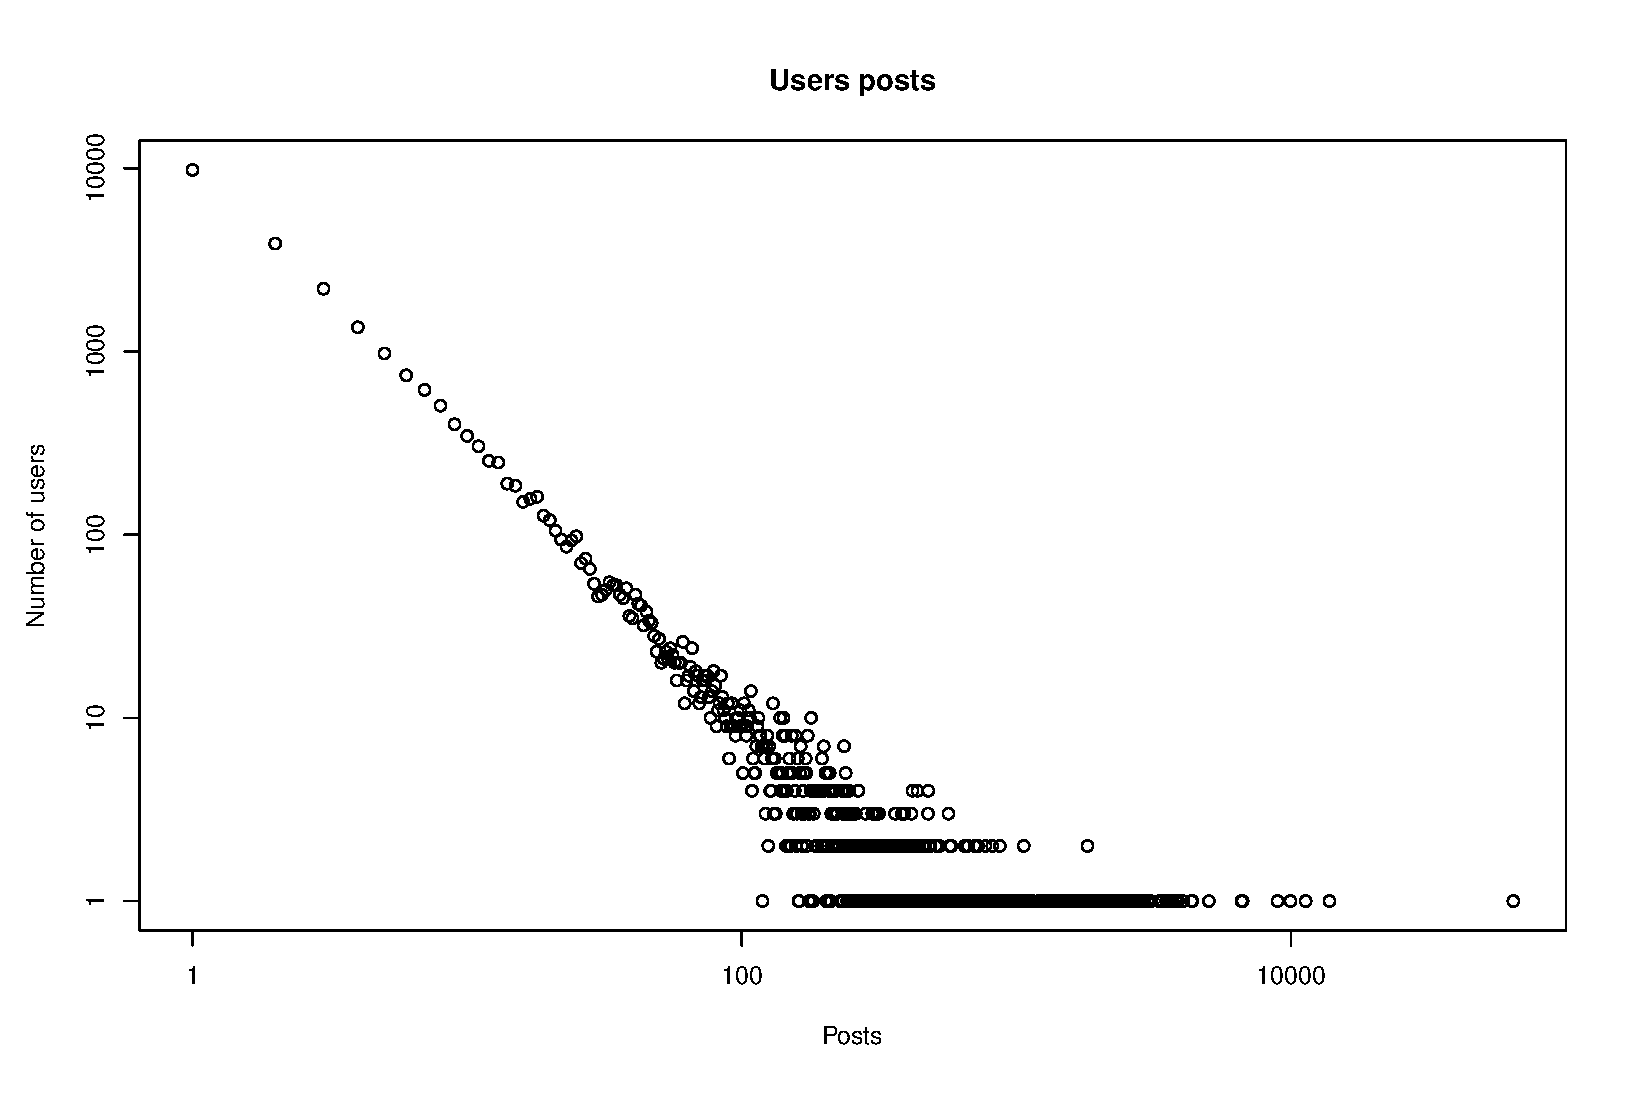
\includegraphics[width=0.5\textwidth]{users_posts}%
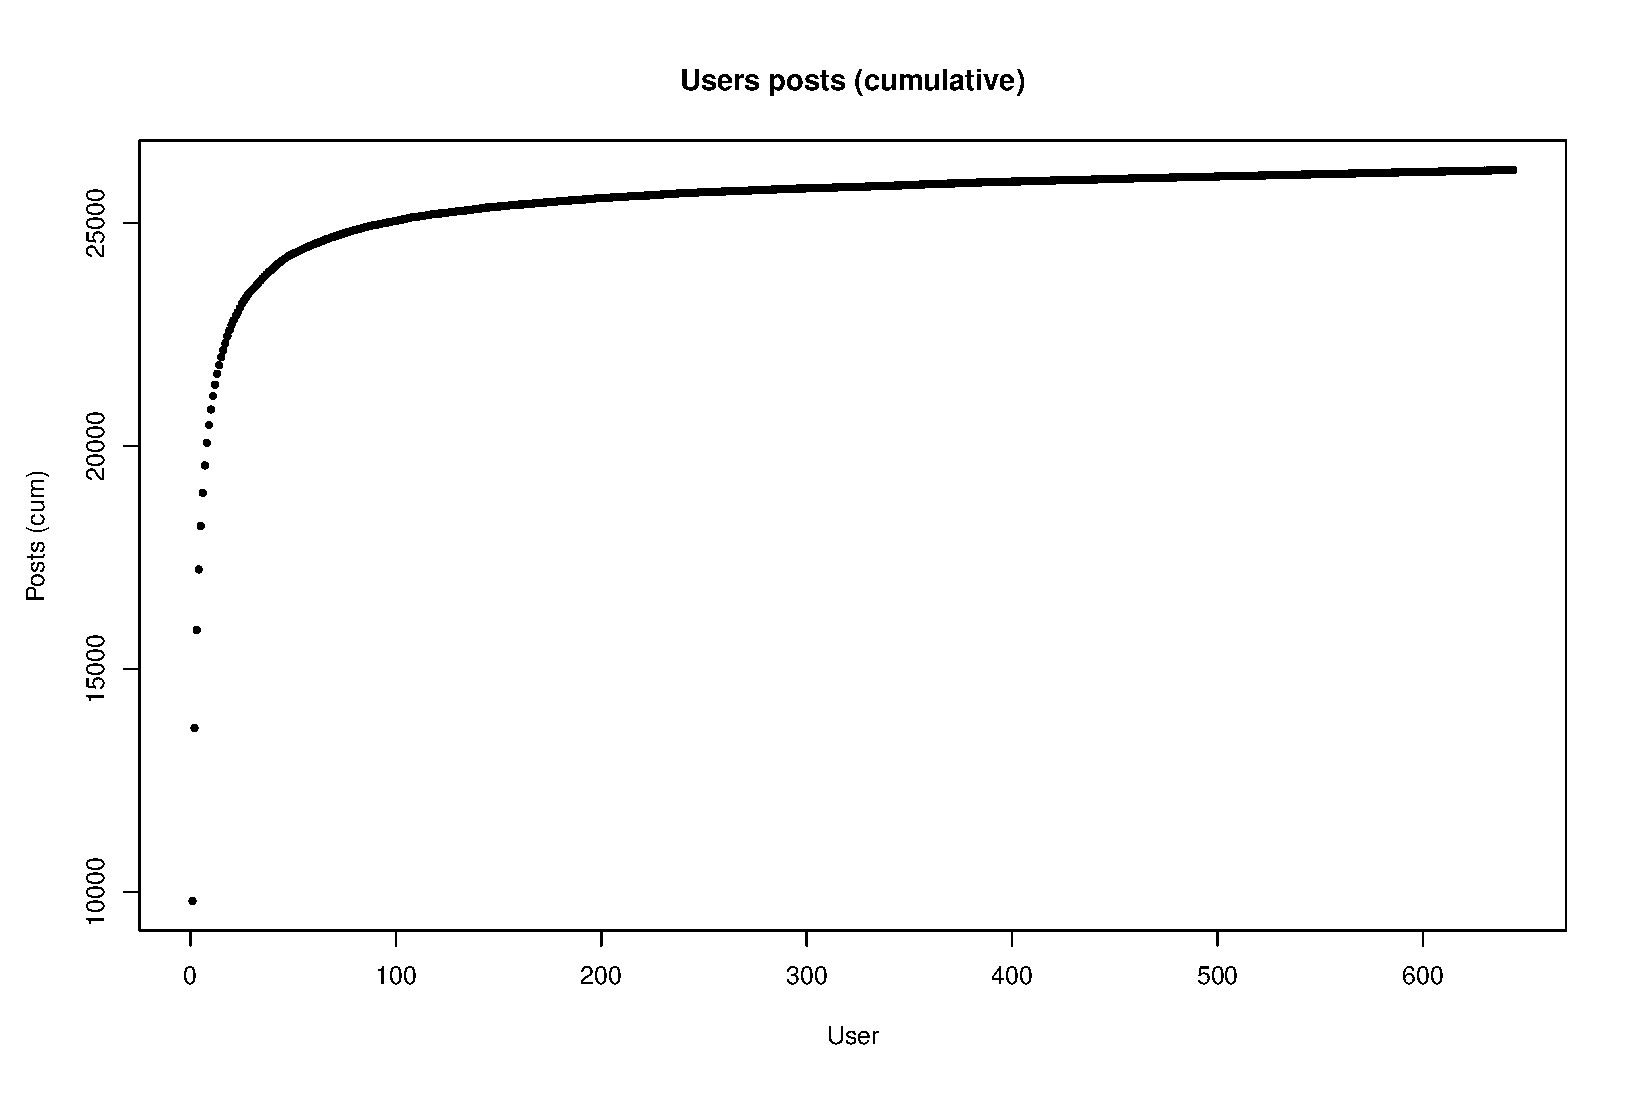
\includegraphics[width=0.5\textwidth]{users_posts_cum}
\caption{Log-log and cumulative distributions and of posts per user.}
\label{fig:podemos_distributions}
\end{figure*}

 %\noindent\textcolor{red}{\rule{16cm}{1mm}}
\subsection{Neighbourhood census}
In this section we analyse the neighbourhood census of our dataset. A counter for every neighbourhood structure is created the first time we detect them. For every post, we extract its neighbourhood (order-based or time-based) and prune it as explained above (Section~\ref{sec:pruning}). Then check whether it is isomorphic to some of the already seen neighbourhoods. If this is the case, then we increment the counter for the neighbourhood previously seen. Otherwise we create a new entry for the current neighbourhood.

\begin{figure*}
	\centering
	\includegraphics[width=0.8\textwidth]{census_orderbased_1}
	%\includegraphics[width=0.8\textwidth]{census_orderbased_2}
	%\includegraphics[width=0.8\textwidth]{census_orderbased_3}
	\caption{Most frequent order-based neighbourhoods with $r=2$ and $n=4$}
	\label{fig:census_orderbased}
\end{figure*}

The census obtained with both type of neighbourhood are similar for the most frequent structures. That means that both kind of neighbourhoods are isomorphic for the most popular discussion structures.



In this section we will build a matrix $M$ for one of the forums of Reddit and then we will cluster users to find groups that have similar preferences over the different types of conversations represented by the neighbourhood structures. 

In order to detect more complex types of neighbourhoods we enlarge the spatial radius to $r=4$. Figure~\ref{fig:neighbourhoods_4_4} shows the eight detected neighbors and their frequency. It is interesting to see different structures like chains or stars where the root node might or might no appear and the ego post is placed at different positions.


\begin{figure*}
	\centering
	\includegraphics[width=0.8\textwidth]{neighbourhoods_3_4_1}
	\includegraphics[width=0.8\textwidth]{neighbourhoods_3_4_2}
	\includegraphics[width=0.8\textwidth]{neighbourhoods_3_4_3}
	\caption{Order-based neighbourhoods with $r=3$ and $n=4$}
	\label{fig:neighbourhoods_4_4}
\end{figure*}


\begin{figure*}
	\centering
	\includegraphics[width=0.8\textwidth]{neighbourhoods_time_1}
	\includegraphics[width=0.8\textwidth]{neighbourhoods_time_2}
	%\includegraphics[width=0.8\textwidth]{neighbourhoods_time_3}
	\caption{Time-based neighbourhoods (most frequent)}
	\label{fig:neighbourhoods_time}
\end{figure*}


Note that some neighbours are still very similar. For instance, \textit{common answer 3} is very close to \textit{common answer 2} in the sense that they both represent the ego post replying to a root post that has one and two replies respectively. It seems a good idea to merge them both since they seem to represent the same type of discussion.

\subsection{Conversation-based clustering of users}

Given the neighbourhoods in which each user participates, we will analyze whether there exists different types of users or all users look similar.

We want to make the analyze independent of the number of posts, and for that we normalize each user feature vector so that features indicate the percentage of posts in this kind of neighbourhood. Moreover, some neighbourhoods are much more common than others due to the nature of the forums. Thus, we normalize and scale the features so that every feature has a global mean 0 and variance 1. User features now represent z-scores, that is, how many standard deviations is this user feature away from the mean.

We use a simple k-means to find the clusters. To decide the number of clusters, we run k-means for k=2,...,25 clusters and look at the Within-Cluster Sum of Squares (Figure~\ref{fig:elbow}) and we chose $k=5$ so that the results are more interpretable.  Figure~\ref{fig:PCA} shows a PCA projection of the users colored by cluster and the distribution of the clusters in every dimension.

\begin{figure*}
	\centering
	\includegraphics[width=1\textwidth]{PCA_cluster_timebased}
	\includegraphics[width=1\textwidth]{PCA_cluster_orderbased}
	\caption{PCA projection of the clusters found and cluster profile in every dimension.}
	\label{fig:PCA}
\end{figure*}

\begin{figure*}
	\centering
	\includegraphics[width=1\textwidth]{PCA_clustering_3_4_order}
	\includegraphics[width=1\textwidth]{clustering_3_4_order}
	\caption{PCA projection of the clusters found and cluster profile in every dimension.}
	\label{fig:PCA}
\end{figure*}


\section{Conclusions}

% use section* for acknowledgment
\section*{Acknowledgment}


The authors would like to thank...





% trigger a \newpage just before the given reference
% number - used to balance the columns on the last page
% adjust value as needed - may need to be readjusted if
% the document is modified later
%\IEEEtriggeratref{8}
% The "triggered" command can be changed if desired:
%\IEEEtriggercmd{\enlargethispage{-5in}}

% references section

% can use a bibliography generated by BibTeX as a .bbl file
% BibTeX documentation can be easily obtained at:
% http://mirror.ctan.org/biblio/bibtex/contrib/doc/
% The IEEEtran BibTeX style support page is at:
% http://www.michaelshell.org/tex/ieeetran/bibtex/
%\bibliographystyle{IEEEtran}
% argument is your BibTeX string definitions and bibliography database(s)
%\bibliography{IEEEabrv,../bib/paper}
%
% <OR> manually copy in the resultant .bbl file
% set second argument of \begin to the number of references
% (used to reserve space for the reference number labels box)
\begin{thebibliography}{1}

\bibitem{IEEEhowto:kopka}
H.~Kopka and P.~W. Daly, \emph{A Guide to \LaTeX}, 3rd~ed.\hskip 1em plus
  0.5em minus 0.4em\relax Harlow, England: Addison-Wesley, 1999.

\end{thebibliography}




% that's all folks
\end{document}


